\subsection{Résultats}

\subsubsection{Détails sur l'implémentation}

L'algorithme de Richardson-Lucy a été implémenté en Python en utilisant la bibliothèque NumPy pour effectuer les calculs matriciels de base, sans recourir à des bibliothèques tierces souvent considérées comme des \textit{boîtes noires}. Cependant, pour des raisons de performance, la bibliothèque SciPy a été utilisée pour les calculs de convolution. Les étapes suivantes ont été suivies :

\begin{itemize}
    \item Les images floues ont été générées en utilisant la fonction \texttt{scipy.signal.convolve2d} avec un noyau de convolution approprié.
    \item Ces images floues ont ensuite été défloutées en appliquant l'algorithme de Richardson-Lucy avec un nombre variable d'itérations.
    \item Les images traitées ont été enregistrées au format PNG pour une visualisation facile.
\end{itemize}

Ainsi, deux versions de l'implémentation de l'algorithme de Richardson-Lucy ont été réalisées :
\begin{itemize}
    \item Une version manuelle, qui ne bénéficie pas des optimisations et est donc plus lente.
    \item Une version rapide (\textit{fast}), qui utilise la bibliothèque SciPy pour les calculs de convolution, offrant ainsi des performances nettement supérieures.
\end{itemize}

La différence de performance entre ces deux versions est significative, la version rapide étant beaucoup plus efficace que la version manuelle.

\subsubsection{Petite précision sur le noyau de convolution}

Par ailleurs, plutôt que le PSF, un noyau de convolution a été utilisé pour générer les images floues. Cela a permis de simuler le flou sans avoir besoin de connaître la PSF exacte.

\subsubsection{Images Originales}

\begin{figure}[h!]
    \centering
    \begin{minipage}[b]{0.45\textwidth}
        \centering
        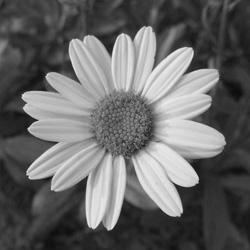
\includegraphics[width=0.8\textwidth]{images/originals/flower.jpg}
        \caption*{(1) Fleur (niveaux de gris)}
    \end{minipage}
    \begin{minipage}[b]{0.45\textwidth}
        \centering
        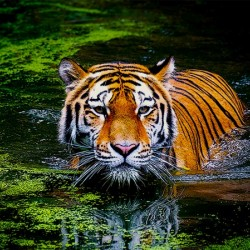
\includegraphics[width=0.8\textwidth]{images/originals/tiger.jpeg}
        \caption*{(2) Tigre}
    \end{minipage}
\end{figure}

\newpage
\subsubsection{Images Traitées}

\subsubsection*{(1) Fleur (niveaux de gris)}

\begin{table}[h!]
    \centering
    \captionsetup{justification=centering}
    \caption*{Images Floutées}
    \begin{tabular}{>{\centering\arraybackslash} m{2cm} >{\centering\arraybackslash} m{2cm} >{\centering\arraybackslash} m{2cm} >{\centering\arraybackslash} m{2cm} >{\centering\arraybackslash} m{2cm} >{\centering\arraybackslash} m{2cm} >{\centering\arraybackslash} m{2cm}}
        \textbf{Average 3x3}                                                                   & \textbf{Average 5x5} & \textbf{Average 11x11} & \textbf{Gaussian 3x3, sigma: 1.0} & \textbf{Gaussian 3x3, sigma: 2.0} & \textbf{Gaussian 5x5, sigma: 1.0} & \textbf{Gaussian 5x5, sigma: 2.0} \\
        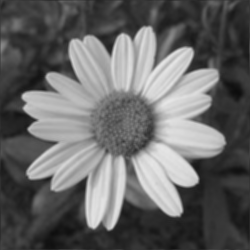
\includegraphics[width=2cm]{images/processed/flower/average_3x3/blurred.png}           &
        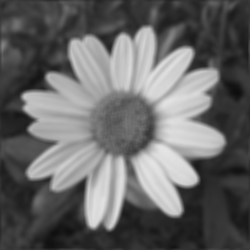
\includegraphics[width=2cm]{images/processed/flower/average_5x5/blurred.png}           &
        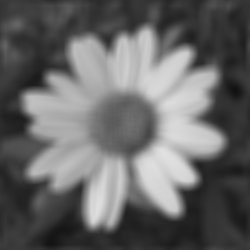
\includegraphics[width=2cm]{images/processed/flower/average_11x11/blurred.png}         &
        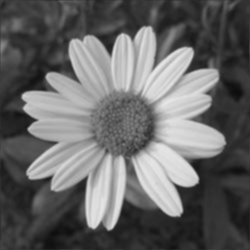
\includegraphics[width=2cm]{images/processed/flower/gaussian_3x3_sigma1.0/blurred.png} &
        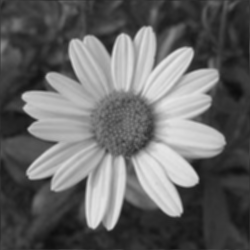
\includegraphics[width=2cm]{images/processed/flower/gaussian_3x3_sigma2.0/blurred.png} &
        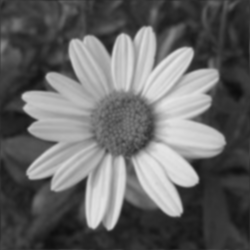
\includegraphics[width=2cm]{images/processed/flower/gaussian_5x5_sigma1.0/blurred.png} &
        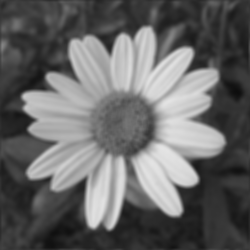
\includegraphics[width=2cm]{images/processed/flower/gaussian_5x5_sigma2.0/blurred.png}                                                                                                                                                                                                 \\
    \end{tabular}
\end{table}

\begin{table}[h!]
    \centering
    \captionsetup{justification=centering}
    \caption*{Images Défloutées - 5 Itérations}
    \begin{tabular}{>{\centering\arraybackslash} m{2cm} >{\centering\arraybackslash} m{2cm} >{\centering\arraybackslash} m{2cm} >{\centering\arraybackslash} m{2cm} >{\centering\arraybackslash} m{2cm} >{\centering\arraybackslash} m{2cm} >{\centering\arraybackslash} m{2cm}}
        \textbf{Average 3x3}                                                                            & \textbf{Average 5x5} & \textbf{Average 11x11} & \textbf{Gaussian 3x3, sigma: 1.0} & \textbf{Gaussian 3x3, sigma: 2.0} & \textbf{Gaussian 5x5, sigma: 1.0} & \textbf{Gaussian 5x5, sigma: 2.0} \\
        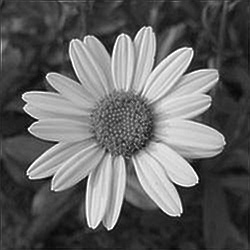
\includegraphics[width=2cm]{images/processed/flower/average_3x3/unblurred_5-iter.png}           &
        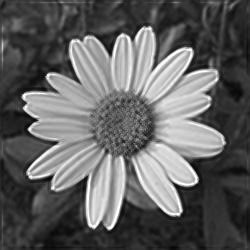
\includegraphics[width=2cm]{images/processed/flower/average_5x5/unblurred_5-iter.png}           &
        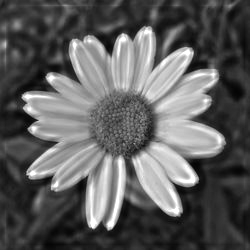
\includegraphics[width=2cm]{images/processed/flower/average_11x11/unblurred_5-iter.png}         &
        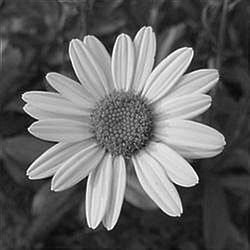
\includegraphics[width=2cm]{images/processed/flower/gaussian_3x3_sigma1.0/unblurred_5-iter.png} &
        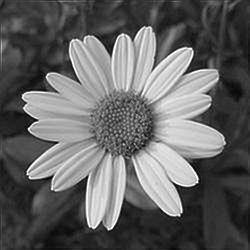
\includegraphics[width=2cm]{images/processed/flower/gaussian_3x3_sigma2.0/unblurred_5-iter.png} &
        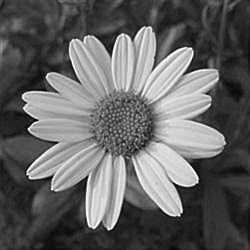
\includegraphics[width=2cm]{images/processed/flower/gaussian_5x5_sigma1.0/unblurred_5-iter.png} &
        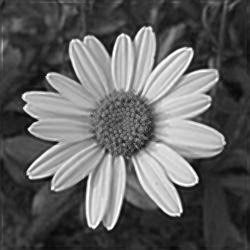
\includegraphics[width=2cm]{images/processed/flower/gaussian_5x5_sigma2.0/unblurred_5-iter.png}                                                                                                                                                                                                 \\
    \end{tabular}
\end{table}

\begin{table}[h!]
    \centering
    \captionsetup{justification=centering}
    \caption*{Images Défloutées - 10 Itérations}
    \begin{tabular}{>{\centering\arraybackslash} m{2cm} >{\centering\arraybackslash} m{2cm} >{\centering\arraybackslash} m{2cm} >{\centering\arraybackslash} m{2cm} >{\centering\arraybackslash} m{2cm} >{\centering\arraybackslash} m{2cm} >{\centering\arraybackslash} m{2cm}}
        \textbf{Average 3x3}                                                                             & \textbf{Average 5x5} & \textbf{Average 11x11} & \textbf{Gaussian 3x3, sigma: 1.0} & \textbf{Gaussian 3x3, sigma: 2.0} & \textbf{Gaussian 5x5, sigma: 1.0} & \textbf{Gaussian 5x5, sigma: 2.0} \\
        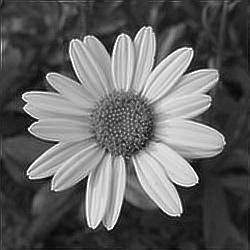
\includegraphics[width=2cm]{images/processed/flower/average_3x3/unblurred_10-iter.png}           &
        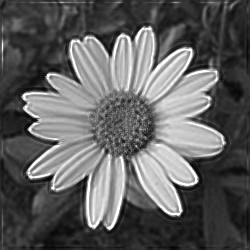
\includegraphics[width=2cm]{images/processed/flower/average_5x5/unblurred_10-iter.png}           &
        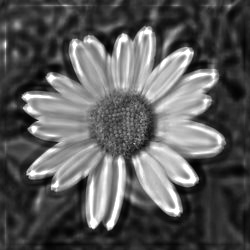
\includegraphics[width=2cm]{images/processed/flower/average_11x11/unblurred_10-iter.png}         &
        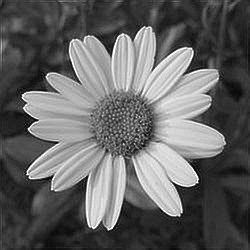
\includegraphics[width=2cm]{images/processed/flower/gaussian_3x3_sigma1.0/unblurred_10-iter.png} &
        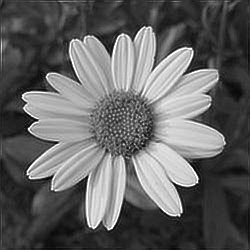
\includegraphics[width=2cm]{images/processed/flower/gaussian_3x3_sigma2.0/unblurred_10-iter.png} &
        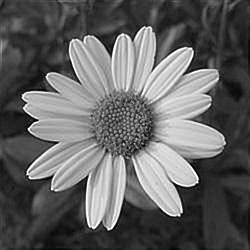
\includegraphics[width=2cm]{images/processed/flower/gaussian_5x5_sigma1.0/unblurred_10-iter.png} &
        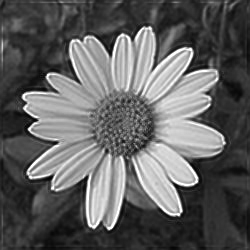
\includegraphics[width=2cm]{images/processed/flower/gaussian_5x5_sigma2.0/unblurred_10-iter.png}                                                                                                                                                                                                 \\
    \end{tabular}
\end{table}

\begin{table}[h!]
    \centering
    \captionsetup{justification=centering}
    \caption*{Images Défloutées - 15 Itérations}
    \begin{tabular}{>{\centering\arraybackslash} m{2cm} >{\centering\arraybackslash} m{2cm} >{\centering\arraybackslash} m{2cm} >{\centering\arraybackslash} m{2cm} >{\centering\arraybackslash} m{2cm} >{\centering\arraybackslash} m{2cm} >{\centering\arraybackslash} m{2cm}}
        \textbf{Average 3x3}                                                                             & \textbf{Average 5x5} & \textbf{Average 11x11} & \textbf{Gaussian 3x3, sigma: 1.0} & \textbf{Gaussian 3x3, sigma: 2.0} & \textbf{Gaussian 5x5, sigma: 1.0} & \textbf{Gaussian 5x5, sigma: 2.0} \\
        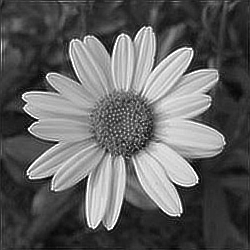
\includegraphics[width=2cm]{images/processed/flower/average_3x3/unblurred_15-iter.png}           &
        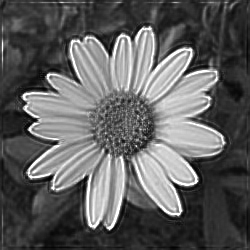
\includegraphics[width=2cm]{images/processed/flower/average_5x5/unblurred_15-iter.png}           &
        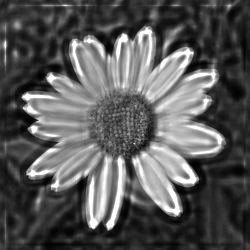
\includegraphics[width=2cm]{images/processed/flower/average_11x11/unblurred_15-iter.png}         &
        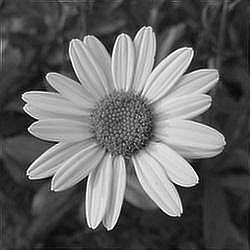
\includegraphics[width=2cm]{images/processed/flower/gaussian_3x3_sigma1.0/unblurred_15-iter.png} &
        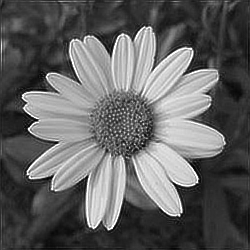
\includegraphics[width=2cm]{images/processed/flower/gaussian_3x3_sigma2.0/unblurred_15-iter.png} &
        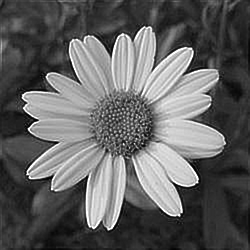
\includegraphics[width=2cm]{images/processed/flower/gaussian_5x5_sigma1.0/unblurred_15-iter.png} &
        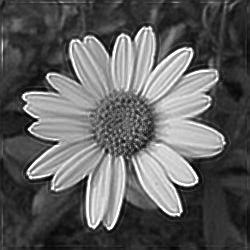
\includegraphics[width=2cm]{images/processed/flower/gaussian_5x5_sigma2.0/unblurred_15-iter.png}                                                                                                                                                                                                 \\
    \end{tabular}
\end{table}

\newpage
\subsubsection*{(2) Tigre}

\begin{table}[h!]
    \centering
    \captionsetup{justification=centering}
    \caption*{Images Floutées}
    \begin{tabular}{>{\centering\arraybackslash} m{2cm} >{\centering\arraybackslash} m{2cm} >{\centering\arraybackslash} m{2cm} >{\centering\arraybackslash} m{2cm} >{\centering\arraybackslash} m{2cm} >{\centering\arraybackslash} m{2cm} >{\centering\arraybackslash} m{2cm}}
        \textbf{Average 3x3}                                                                  & \textbf{Average 5x5} & \textbf{Average 11x11} & \textbf{Gaussian 3x3, sigma: 1.0} & \textbf{Gaussian 3x3, sigma: 2.0} & \textbf{Gaussian 5x5, sigma: 1.0} & \textbf{Gaussian 5x5, sigma: 2.0} \\
        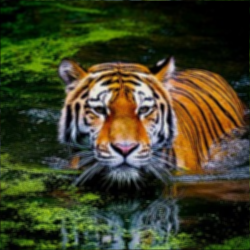
\includegraphics[width=2cm]{images/processed/tiger/average_3x3/blurred.png}           &
        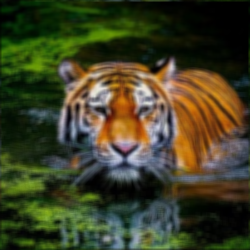
\includegraphics[width=2cm]{images/processed/tiger/average_5x5/blurred.png}           &
        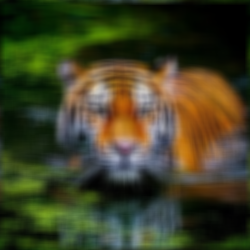
\includegraphics[width=2cm]{images/processed/tiger/average_11x11/blurred.png}         &
        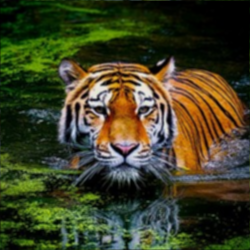
\includegraphics[width=2cm]{images/processed/tiger/gaussian_3x3_sigma1.0/blurred.png} &
        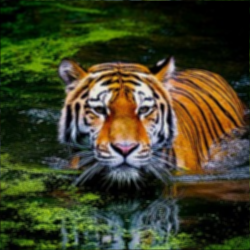
\includegraphics[width=2cm]{images/processed/tiger/gaussian_3x3_sigma2.0/blurred.png} &
        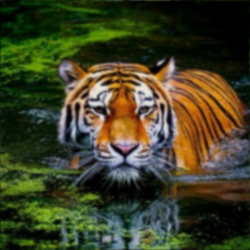
\includegraphics[width=2cm]{images/processed/tiger/gaussian_5x5_sigma1.0/blurred.png} &
        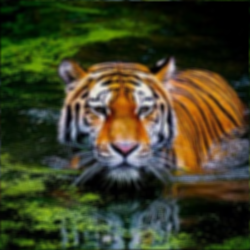
\includegraphics[width=2cm]{images/processed/tiger/gaussian_5x5_sigma2.0/blurred.png}                                                                                                                                                                                                 \\
    \end{tabular}
\end{table}

\begin{table}[h!]
    \centering
    \captionsetup{justification=centering}
    \caption*{Images Défloutées - 5 Itérations}
    \begin{tabular}{>{\centering\arraybackslash} m{2cm} >{\centering\arraybackslash} m{2cm} >{\centering\arraybackslash} m{2cm} >{\centering\arraybackslash} m{2cm} >{\centering\arraybackslash} m{2cm} >{\centering\arraybackslash} m{2cm} >{\centering\arraybackslash} m{2cm}}
        \textbf{Average 3x3}                                                                           & \textbf{Average 5x5} & \textbf{Average 11x11} & \textbf{Gaussian 3x3, sigma: 1.0} & \textbf{Gaussian 3x3, sigma: 2.0} & \textbf{Gaussian 5x5, sigma: 1.0} & \textbf{Gaussian 5x5, sigma: 2.0} \\
        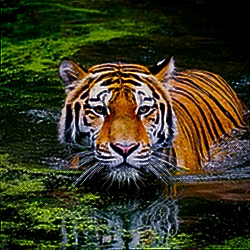
\includegraphics[width=2cm]{images/processed/tiger/average_3x3/unblurred_5-iter.png}           &
        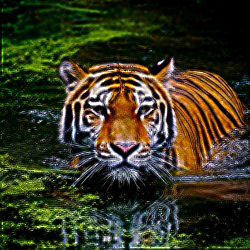
\includegraphics[width=2cm]{images/processed/tiger/average_5x5/unblurred_5-iter.png}           &
        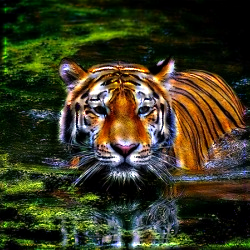
\includegraphics[width=2cm]{images/processed/tiger/average_11x11/unblurred_5-iter.png}         &
        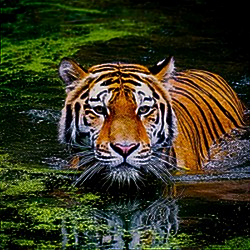
\includegraphics[width=2cm]{images/processed/tiger/gaussian_3x3_sigma1.0/unblurred_5-iter.png} &
        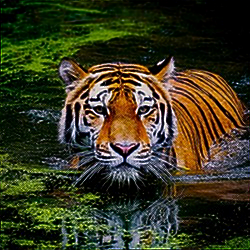
\includegraphics[width=2cm]{images/processed/tiger/gaussian_3x3_sigma2.0/unblurred_5-iter.png} &
        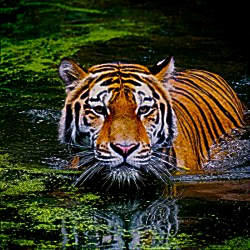
\includegraphics[width=2cm]{images/processed/tiger/gaussian_5x5_sigma1.0/unblurred_5-iter.png} &
        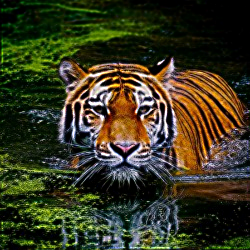
\includegraphics[width=2cm]{images/processed/tiger/gaussian_5x5_sigma2.0/unblurred_5-iter.png}                                                                                                                                                                                                 \\
    \end{tabular}
\end{table}

\begin{table}[h!]
    \centering
    \captionsetup{justification=centering}
    \caption*{Images Défloutées - 10 Itérations}
    \begin{tabular}{>{\centering\arraybackslash} m{2cm} >{\centering\arraybackslash} m{2cm} >{\centering\arraybackslash} m{2cm} >{\centering\arraybackslash} m{2cm} >{\centering\arraybackslash} m{2cm} >{\centering\arraybackslash} m{2cm} >{\centering\arraybackslash} m{2cm}}
        \textbf{Average 3x3}                                                                            & \textbf{Average 5x5} & \textbf{Average 11x11} & \textbf{Gaussian 3x3, sigma: 1.0} & \textbf{Gaussian 3x3, sigma: 2.0} & \textbf{Gaussian 5x5, sigma: 1.0} & \textbf{Gaussian 5x5, sigma: 2.0} \\
        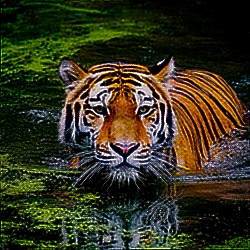
\includegraphics[width=2cm]{images/processed/tiger/average_3x3/unblurred_10-iter.png}           &
        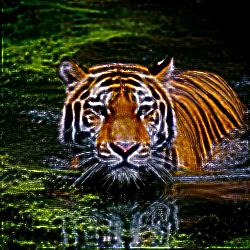
\includegraphics[width=2cm]{images/processed/tiger/average_5x5/unblurred_10-iter.png}           &
        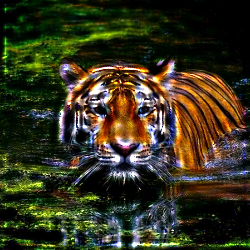
\includegraphics[width=2cm]{images/processed/tiger/average_11x11/unblurred_10-iter.png}         &
        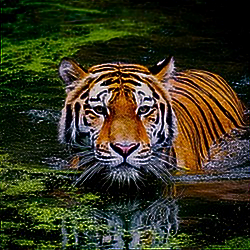
\includegraphics[width=2cm]{images/processed/tiger/gaussian_3x3_sigma1.0/unblurred_10-iter.png} &
        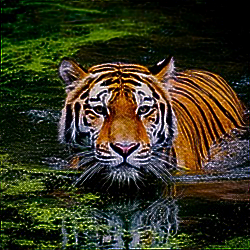
\includegraphics[width=2cm]{images/processed/tiger/gaussian_3x3_sigma2.0/unblurred_10-iter.png} &
        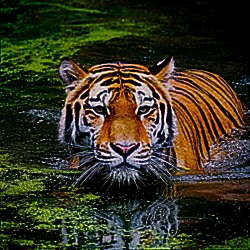
\includegraphics[width=2cm]{images/processed/tiger/gaussian_5x5_sigma1.0/unblurred_10-iter.png} &
        \includegraphics[width=2cm]{images/processed/tiger/gaussian_5x5_sigma2.0/unblurred_10-iter.png}                                                                                                                                                                                                 \\
    \end{tabular}
\end{table}

\begin{table}[h!]
    \centering
    \captionsetup{justification=centering}
    \caption*{Images Défloutées - 15 Itérations}
    \begin{tabular}{>{\centering\arraybackslash} m{2cm} >{\centering\arraybackslash} m{2cm} >{\centering\arraybackslash} m{2cm} >{\centering\arraybackslash} m{2cm} >{\centering\arraybackslash} m{2cm} >{\centering\arraybackslash} m{2cm} >{\centering\arraybackslash} m{2cm}}
        \textbf{Average 3x3}                                                                            & \textbf{Average 5x5} & \textbf{Average 11x11} & \textbf{Gaussian 3x3, sigma: 1.0} & \textbf{Gaussian 3x3, sigma: 2.0} & \textbf{Gaussian 5x5, sigma: 1.0} & \textbf{Gaussian 5x5, sigma: 2.0} \\
        \includegraphics[width=2cm]{images/processed/tiger/average_3x3/unblurred_15-iter.png}           &
        \includegraphics[width=2cm]{images/processed/tiger/average_5x5/unblurred_15-iter.png}           &
        \includegraphics[width=2cm]{images/processed/tiger/average_11x11/unblurred_15-iter.png}         &
        \includegraphics[width=2cm]{images/processed/tiger/gaussian_3x3_sigma1.0/unblurred_15-iter.png} &
        \includegraphics[width=2cm]{images/processed/tiger/gaussian_3x3_sigma2.0/unblurred_15-iter.png} &
        \includegraphics[width=2cm]{images/processed/tiger/gaussian_5x5_sigma1.0/unblurred_15-iter.png} &
        \includegraphics[width=2cm]{images/processed/tiger/gaussian_5x5_sigma2.0/unblurred_15-iter.png}                                                                                                                                                                                                 \\
    \end{tabular}
\end{table}
